\documentclass{article}
%\usepackage[utf8]{inputenc}
\usepackage{graphicx}
\usepackage{hyperref}
\usepackage{enumerate}
\usepackage{amsmath}
\usepackage{amsfonts}
\usepackage{hyperref}

\setlength\parindent{0pt}

\title{A Multi-Class Classifier for Amazon Reviews}
\author{Arjun Mody \& Michael Zochowski}
\date{May 4, 2014}

\begin{document}

\maketitle
\section{Abstract}
We examine the problem of classifying reviews into a quantitative, multilevel rating (1 through 5 stars)
based on the sentiment expressed in the review�s language through machine learning techniques.
We focus on Amazon reviews for software products and build SVMs to predict the assigned rating
based on the review text.  We consider two methods for multi-class classification - the one-vs-all strategy where
5 SVMs compare a rating vs all other ratings, and pairwise one-vs-one strategy where 10 SVMs
compare each pair of ratings.  We additionally consider the selection of features, including the
use of $n$-grams, phrases of length $n$ words.  Factors considered are size of the learning set,
the number of features from each category, the removal of common words,
the minimum frequency in the corpus of the learning set to be considered, the highest cardinality of $n$-grams 
to include, and how to parse the text.  We finally construct an SVM set that will give the best
prediction results (given time limitations) based on these parameters, with a mean squared error of 2.34 and a correct prediction rate of $50.4\%$
\section{Motivation}
The problem of classifying into multiple categories is an interesting extension of simple classification into two categories.  There are a variety methods to deal with this complication, but none is obviously better than the others.  Thus, building a method to classify Amazon reviews into one of five categories (1 star to 5 star) can give insights into this issue.\\

An additional wrinkle presented by classification of Amazon reviews is that the categories are ordered.  Unlike unordered categories, such as (cat, dog, sheep, pig, horse), the rating categories $(1,2,3,4,5)$ have an inherent order.  Thus, it is better to predict 2 stars for a 1 star review rather than 5 stars, while it is not obviously better to predict cat than dog if the object is actually a pig.  This issue is not confronted in two category classification, and how to deal with it gives the problem further depth.\\

While the ability to classify Amazon reviews itself has little direct value, the methods used have a variety of applications. For example, an investing strategy that parses and categorizes news articles about a specific company will be much more effective if it has the capacity to offer a gradient of ratings rather than just ``positive" or ``negative".  The methods could also be used to assign a rating to social media posts about a product where a rating is not given (such as on Twitter).

\section{Data}
For this project, we use a collection of Amazon reviews regarding software products. The data set can be found through SNAP (Stanford Network Analysis Project) at the following link (https://snap.stanford.edu/data/web-Amazon-links.html) under ``Software Reviews."\\\\
Each item in our data set contains the following fields:\\
\begin{center}
\begin{tabular}{|c|c|}\hline
 Field & Example\\\hline
product/productId & B00006HAXW\\\hline
review/userId & A1RSDE90N6RSZF\\\hline
review/profileName & Michael C. Zochowski\\\hline
review/helpfulness & 121/221\\\hline
review/score & 5.0\\\hline
review/time & 1042502400\\\hline
review/summary & Enjoyable\\\hline
review/text & My five-year-old had a great time\\ & playing this computer game.\\\hline
\end{tabular}
\end{center}
Rating is an integer between 1.0 and 5.0. Review helpfulness denotes that $X$ out of $Y$ found the review helpful. Review summary is the title that appears above the review text when users are browsing through product reviews.
We compute some simple summary statistics on our data set, given in the following table:
\begin{center}
\begin{tabular}{|c|c|}\hline
Number of Reviews & 95,084\\\hline
Avg. Rating & 3.3008 \\\hline
Avg. Helpfulness & 9.65 / 11.98\\\hline
Avg. Helpfulness \% & 0.769\\\hline
Avg. No. Words / Review & 127.1\\\hline
\end{tabular}
\end{center}
Note that the average helpfulness percentage is slightly lower than the average numerator value (9.65) divided by the average denominator value (11.98) since we count reviews as 0/1 if zero people out of zero find the review helpful.\\\\
Below is the distribution of ratings:
\begin{center}
\begin{tabular}{c|c}
 Rating & Frequency \\\hline
 $\star$ & 0.2713\\
 $\star$$\star$ & 0.8493\\
 $\star$$\star$$\star$ & 0.0935\\
 $\star$$\star$$\star$$\star$ & 0.1721\\
 $\star$$\star$$\star$$\star$$\star$ & 0.3781\\
\end{tabular}
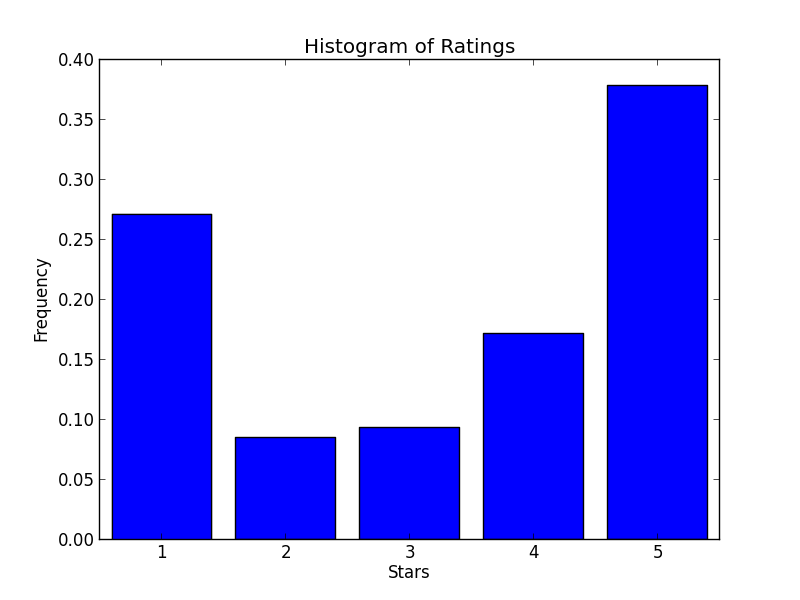
\includegraphics[scale=0.5]{software-score-hist.png}
\end{center}

\section{Feature Selection}
The most important part of building the SVMs is in performing feature selection. Since the learning set can be quite large, and solving LPs of high dimension can be challenging, selecting a small but useful set of features for the SVMs is a crucial step. We used the following method to select features. First, we parsed out puncuation from the learning set and split on words. Then we remove some number (a parameter to our SVM) of most commonly occuring words in the English language. Then we compute the Z-score of words for each category, and take some number (another parameter) of words with the highest Z-score for each category. We elaborate on stemming and Z-scores below. We also did the above process for 2-grams and 3-grams, which are simply pairs of words and triplets of words that appear in a row. For instance, the phrase ``not good" is much more informative than ``not" and ``good" independently, which is the kind of intuition that we want to be able to capture.
\subsection{Stemming}
``Stemming" is a process in natural language processing by which words are reduced to their root, or stem, so that they are not ``double-counted" when computing the frequency of words in a review, for instance. For example, the words ``running" and ``runs" might be reduced to ``run." We initially used the python library \texttt{stemming 1.0} to pre-process reviews, but this proved to be too slow, so we used a C-implementation instead.\\\\
We initially also wanted to incorporate a spell checker after stemming, since sometimes stemming reduces a word to something that is not a word (i.e., changing the word easily to easi). However, we could not find a spell checker that was efficient enough to allow us to do extensive testing. We do note, however, that a word that is incorrectly stemmed will only result in false positives rather than false negatives, since any occurence of the incorrectly stemmed word will be stemmed in the same way.
\subsection{Z-scores}
There are many naive approaches to feature selection which include taking simply the most frequent words or those that do not occur in the intersection of the two categories. We use an approach described by Olena Kummer and Jacques Savoy (2012) in which they use the normalized Z-score of different features within a specific category to determine how "confident" they are at predicting the sentiment of a sentence. We adapt a basic version of their method, which is used for binary classification, to our multi-classification problem.\\\\
Let $C$ be the entire corpus of reviews that we are examining for feature selection. Let $S$ be the subset of reviews with a particular label, such as 5-star reviews. Then $\neg S$ is the rest of the reviews, and $C = S\cup \neg S$. Let $f$ be some feature of interest, and $\neg f$ contains all other features. Consider the following table:\\
\begin{center}
\begin{tabular}{|c|c|c|c|}\hline
 & $S$ & $\neg S$ & $C$\\\hline
 $f$ & $a$ & $b$ & $a + b$\\\hline
 $\neg f$ & $c$ & $d$ & $c + d$\\\hline
 & $a + c$ & $b + d$ & $n$\\\hline
\end{tabular}
\end{center}
Here, $a$ is the number of times the feature appears in the subset. $b$ is the number of times the feature appears in the rest of the reviews, and $a + b$ is the number of times it appears in the entire corpus. Thus, $P(f) = (a + b)/n$ is the frequency that $f$ appears at all. Let $n'$ be the number of words in the subset, or $n' = a + c$. Then, we can treat the distribution of $f$ as a binomial distribution where $P(f)$ is the probability of drawing it and $n'$ is the number of trials. Thus, $P(f)\cdot n'$ gives us the expected number of times that $f$ should appear in the subset when using the frequency over the entire corpus. If the value $a - P(f)\cdot n'$, or the difference between the actual number of times that $f$ is observed in $S$ and the expected number of times, is large, then we can be confident that the distribution of $f$ in $S$ differs from its distribution in $C$. We use the following normalized Z-score for a feature:
\[ \text{Z-score}(f) = \frac{a - n'\cdot P(f)}{\sqrt{n'\cdot P(f)\cdot(1 - P(f)}}\]\\
As an example, here are the words with the top-10 Z-scores for one-star reviews:
\begin{center}
\begin{tabular}{c|c}
word & Z-score\\\hline
uninstall & 6.48\\
money & 6.44\\
waste & 6.34\\
tech & 6.12\\
worst & 5.65\\
tri & 5.64\\
symantec & 5.29\\
poor & 5.28\\
custom & 5.19\\
crash & 5.04\\
\end{tabular}
\end{center}
As we can see, the Z-score method seems to work a bit on this data, selecting words such as ``uninstall," ``waste," ``worst," ``poor," and ``crash" for one-star reviews. The other words don't have much explanation for why they would be indicative of a one-star review, however.

\section{SVMs as LPs}
A Support Vector Machine is used to perform binary classification. We are given a set of $n$ observations $(x_i, y_i)\in \mathbb{R}^d\times \{-1, +1\}$, where $x_i$ is a feature vector corresponding to an observation, and $y_i$ is its class / label (binary). The problem at hand is to build a classifier $c:\mathbb{R}^d\rightarrow\{-1, +1\}$ which takes in a feature vector corresponding to some data point, and predicts its label.\\\\
The actual feature vector is constructed using the method in Section 3. Then, to convert a review into a feature vector, we simply count the number of times that each feature occurs in the review and these become the components of the vector corresponding to our review.\\\\
An SVM classifier, geometrically, is a hyperplane defined by a vector $w\in\mathbb{R}^d$ and constant $b\in\mathbb{R}$ such that
 \begin{displaymath}
   c_{w, b}(x) = \left\{
     \begin{array}{lr}
       -1 & : w^Tx - b\geq +1\\
       +1 & : w^Tx - b\leq -1
     \end{array}
   \right.
\end{displaymath} 
As we learned in class, if we use the $l_1$ norm ($||w||_1 = \sum |w_i|$), we can formulate the problem of finding an optimal SVM for a set of data as a linear program. In particular, we want to minimize the margin, or the distance from the hyerplane to the closest point on either side, which is equivalent to minimizing the norm of the vector $w$ (proven in class). We also use the soft-margin relaxation technique, which allows us to find a hyerplane even if the data are not truly separable (i.e., the smallest convex sets that contain the two classes intersect). The error for each datapoint in the learning set is denoted by $\xi_i$. Finally, we linearize the absolute value function in the objective value. Putting these all together, we get the following LP:
\begin{align*}
\min_{w_i^+,w_i^-,b^+,b^-,\xi}\quad & \sum_{i = 1}^d (w_i^+ + w_i^-) + C\sum_{i = 1}^n \xi_i\\
\text{s.t.}\quad & y_i((w^+ - w^-)^Tx_i - (b^+ - b^-))\geq 1 - \xi_i\quad&\forall i\in [n]\\
& w_i^+, w_i^-, b^+, b^-, \xi_i\geq 0\quad&\forall i\in[n]
\end{align*}
The optimal $w$ and $b$ from above give us our SVM.
\section{Extending SVMs to Multi-Class Classification}
In our project, we used SVMs for multi-class classification in the following two ways.
\subsection{One-vs-All}
In the one-vs-all approach, we build an SVM for each class. Each SVM represents a hyperplane that separates the class from the other classes, i.e. it tells us whether it is more likely that a data point belongs to some class or to any other class. Then, to classify, the distance of a point from each SVM is computed, and whichever SVM for which the data point is the ``most positive" (i.e. on the side of that rating versus everything else) is the SVM that we choose.
\subsection{Pairwise}
In the pairwise approach, we construct $\sum_{i = 1}^{n - 1} (i)$ SVMs if we have $n$ classes. That is, we construct $4 + 3 + 2 + 1 = 10$ SVMs for our 5-class problem, in which each SVM does a pairwise comparison (i.e., one star vs three star). The learning sets have to be different for each SVM now, since they only include reviews that are of the two classes being separated. Then, to classify a point, each of the SVMs is used, and a ``vote" happens, whereby the class. Ties are broken based on the confidence scores of the SVMs.\\\\
We hypothesize that the pairwise approach will perform better, since it takes the inherent linearity in the classification problem into account. For instance, 1-star reviews should be closer to 2-star reviews than to 5-star reviews. In a sense, building a 3-vs-all classifier might not make much sense, because it's possible that the 3-star reviews are in the ``middle" of whatever space the data live in, and are not very separable from both 1-star reviews and 5-star reviews by the same hyerplane. Building a hyperplane for each classification problem as is done in the pairwise approach takes this into account, whereas the one-vs-all approach cannot.
\section{Results}
All results are when our classifier runs on 1000 predictions, and we measured the time it took to construct the learning dictionaries, the mean square error of the predictions (MSE), and the percentage of correct predictions. The mean square error for $N$ predictions, where $X_i$ is the predicted value and $Y_i$ is the true value, is given by
\[\frac{1}{N}\sum_{i = 1}^{N} (X_i - Y_i)^2\]
and to us seems like the most reasonable metric for accuracy. \\\\
We varied the following parameters when collecting results: Type (one-vs-all or pairwise), LearnSet (the number of reviews in the learning set), FeatureCt (the number of features used per category, based on top Z-score), MaxN (maximum length of $n$-grams used), MinCount (the minimum number of times a phrase must have appeared in the learning set to be considered a feature), $C$ (the cost of misclassificaiton in the optimization problem), and NCommon (the number of most common English words removed from the feature set).\\\\
First, we tested the effect of changing $C$ (with LearnSet = 1000, FeatureCt = 100, MinCount = 20, NCommon = 150):
\begin{center}
\begin{tabular}{c|c|c|c|c}
Type & MaxN & $C$ & MSE & \% Correct \\\hline
Pairwise & 1 & 100 & 3.111 &	0.433\\
Pairwise & 1 & 5 &3.207 &	0.418\\
\textbf{Pairwise} & \textbf{1} & \textbf{1} &\textbf{2.816} &	\textbf{0.4702}\\
Pairwise & 2 & 10 & 2.838	&0.437\\
Pairwise & 2 & 1 & 2.957	&0.474
\end{tabular}
\end{center}
To our surprise, setting the value of $C$ to be low gave us the best results for 1-grams. This means that the objective function does not need to heavily penalize misclassifications in order to find a good hyperplane. However, since the result was not true for 2-grams as well, we think $C$ has not much measureable effect on the accuracy of our classifier, and thus let it be 10 for the majority of our tests.\\\\
Next, we explored the effect of changing NCommon (with LearnSet = 1000, FeatureCt = 100, MinCount = 20, $C$ = 10):
\begin{center}
\begin{tabular}{c|c|c|c|c}
Type & MaxN & NCommon & MSE & \% Correct \\\hline
\textbf{Pairwise} & \textbf{1} & \textbf{0}	&	\textbf{2.799}	& \textbf{0.451}\\
Pairwise & 1 &50	&	2.945	& 0.431\\
Pairwise & 1 &200	&	3.019	& 0.406\\
\end{tabular}
\end{center}

We were surprised again that extracting common words seemed to improve the performance for 1-gram pairwise classification.\\\\
Next, we varied MaxN and Type (with LearnSet = 1000, FeatureCt = 100, MinCount = 20, $C$ = 10, NCommon = 150):
\begin{center}
\begin{tabular}{c|c|c|c|c}
Type & MaxN & MSE & \% Correct & DictTime (s) \\\hline
One-vs-all & 1 & 3.003	&0.435 & 38.8329\\
One-vs-all &2 & 3.135	&0.432 & 1048.5652\\
One-vs-all &3 & 3.069	&0.423 & 7295.9174\\
Pairwise &1 & 3.111	& 0.433 & 19.6172\\
\textbf{Pairwise} & \textbf{2} & \textbf{2.838}	& \textbf{0.437} & \textbf{723.6752}\\
Pairwise &3 & 2.934	&0.426 & 8636.5561
\end{tabular}
\end{center}

We can see that pairwise classification, using 1- and 2-grams had the best performance with an MSE of 2.838. We can see that there is a dramatic increase in the amount of time it takes to construct the learning dictionaries when longer $n$-grams are considered. Even though for every word in a review, there are two 2-grams (and three 3-grams), there are many more duplicates of individual words than 2-grams, which means that the number of features which must be considered is quite large.\\\\
After deciding that 2-gram pairwise classification gave the best results, we optimized for MinCount (with LearnSet = 1000, FeatureCt = 100, $C$ = 10, NCommon = 150):
\begin{center}
\begin{tabular}{c|c|c|c|c}
Type & MaxN & MinCount & MSE & \% Correct \\\hline
Pairwise & 2 & 20 & 2.838	&0.437\\
Pairwise & 2 & 10 & 2.771	&0.425\\
\textbf{Pairwise} & \textbf{2} & \textbf{8} & \textbf{2.756}	&\textbf{0.439}\\
Pairwise & 2 & 7 & 2.912	&0.425\\
\end{tabular}
\end{center}
After concluding that MinCount = 8 worked the best, we finally experimented with changing the size of the learning set and the number of features used to try and find the best classifier that we can given our model. The results are (with Type = pairwise, MaxN = 2, MinCount = 8, $C$ = 10, NCommon = 150):
\begin{center}
\begin{tabular}{c|c|c|c|c}
LearnSet & FeatureCt & MSE & \% Correct & DictTime (s) \\\hline
1200 & 200 & 2.86	& 0.448 & 1072.21\\
1500 & 200 & 2.5576	& 0.4784 & 1823.79\\
2000 & 250 & 2.3578	& 0.4828 & 2784.65\\
\textbf{2500} & \textbf{1000} & \textbf{2.34} & \textbf{0.504} & \textbf{4732.06}
\end{tabular}
\end{center}

As we can see, increasing the number of features helps dramatically in decreasing the MSE, but doing so takes a long time to run (the last trial took almost an hour and a half to just construct the learning dictionaries. 

\subsection{Best Results}
\begin{center}

\begin{tabular}{c|c}
Parameter & Value\\\hline
LearnSet & 2500\\
FeatureCt & 1000\\
Type & Pairwise\\
MaxN & 2\\
MinCount & 8\\
$C$ & 10\\
NCommon & 150\\
\textbf{MSE} & \textbf{2.34}\\
\textbf{\% Correct}& \textbf{0.504}
\end{tabular}
\end{center}
The above parameters give the SVM which yielded the best performance for us. It classifies just above half of the reviews correctly, while achiving an MSE of 2.34, which corresponds to a standard error of $\sqrt{2.34} = 1.51$ stars off in its predictions. Given how noisy the data is, and that there may not be clear delineations between 3 and 4 star reviews, for instance, we think that being 1.5 stars off in classification on average is a good benchmark to have achieved.
\subsection{Examples of Misclassifications}
While we achieve a low MSE, the program still gives some bad misclassifications.  For example, the following 5 star review has a 1 star prediction:
\begin{quotation}
I am a big graphics person and I have several graphics packages that I am not satisfied with. But when I purchased this I was really impressed with the graphics and the other features as well. I even recommended this software to a friend of mine who is also into graphics pacakages like myself. If I would have found this software before, I would not have wasted the money I spent on the other packages I have. Thanks again. A very satisfied customer.
\end{quotation}
The vote tally for $(1,2,3,4,5)$ was $(4,  2,  1,  0,  3)$.
This review includes several phrases that trips up the SVM-set, including ``not satisfied", ``would not", and ``wasted money".  Nonetheless, 5-star had the second most votes, so the program was not too far off.  Generally, egregious misclassifications followed this same pattern where the review included an opposing experience that constrasted with their experience with the product they are reviewing.\\

Similarly, the following 1 star review was predicted to be 5 star:
\begin{quotation}
This game sucks! I bought it with my last couple of bucks from my birthday and when I went to play it I nearly fainted! I like action games like Battle Arena Toshinden. Not very many people know what that game is but it is one of the best games I own. I ended up giving dogz it to my 3 year old cousin. You cant save either. So every time you turn it on you have to pick a dog name it pick a color and make it like you. There is no level s of play either, just one level the whole time! Take my advise DON'T BUY IT!!:)
\end{quotation}
In this case, the reviewer uses language such as ``like" and ``one of the best games I own" to describe his favorite game in contrast with the game he is reviewing.\\

These type of reviews present the biggest challenge to any machine learning classification approach.  It likely would require significantly more complex methods to identify when a reviewer is discussing another product, if this is at all possible.  When the reviewer sticks to discussing the reviewed product, the program tends to do very well.

\section{Conclusions}
We were able to successfully implement a multi-class classifier that exceeded the $50\%$ correctness threshold and gave a MSE of $2.34$.  Using these same methods, we could construct an even better classifier if we ran the program for several days.  Ultimately, we found that the pairwise one-vs-one approach was superior to the one-vs-all approach in reflecting the ordered nature of the rating categories, and it accordingly gave better results.  Adding bigrams to feature consideration gave a significant improvement to results (along with a large increase in computation time), but trigrams did not give added benefit.  A frequency threshold of 8 and removal of the 150 most common words were also found to improve results.  Other features, such as spelling correction, could have improved results but were computationally impractical.\\

The largest challenge remains reviews that include language contrary to the assigned rating, such as when discussing a contrasting experience with another product.  Furthermore, construction of the SVMs is computationally intensive, with total run times exceeding 1.5 hours for the best configurations we examined, making optimization over parameters challenging.\\

Overall, we believe the model we present is a robust and accurate way of categorizing in an ordered, multi-class framework.

\section{The Code}
The code is hosted on Github: \url{https://github.com/mczochowski/am221-project.git}.\\\\
The relevant code is in the following files:
\begin{itemize}
\item \texttt{svm.py} (\texttt{./python\_svm/}): This file contains our main script to build the SVMs and make predictions using the functions in \texttt{build\_svm.py} and \texttt{predict.py}, respectively. The file has includes the function \texttt{load\_text()}, which loads in the reviews from the raw data file and structures them.  The file can be run with various options, detailed below.\\\\
Usage: \texttt{\textasciitilde\$ .\textbackslash svm.py [-h] [-s] [-p] <numpredictions> [-v] [-t] <type>}:
\begin{itemize}
\item \texttt{-h} (help): Output usage instructions
\item \texttt{-s} (svm): Build the SVMs (takes some time)
\item \texttt{-d} (dictionaries): Re-write the dictionaries
\item \texttt{-p numpredictions} (predict): Make an integer number of predictions.
\item \texttt{-v} (verbose): Output information about each individual prediction, including the predicted rating, the actual rating, and the review text.
\item \texttt{-t type} (type): Set to 0 (default) for one-vs-all prediction, and set to 1 for pairwise prediction.
\end{itemize}
\item \texttt{constants.py}: This file contains relevant constants to run our various scripts (such as the locations of various files).  The relevant constants defined are:
\begin{itemize}
\item \texttt{nl}: The number of reviews to include in the learning set (randomly selected)
\item \texttt{min\_ct}: minimum number of occurrences in corpus to be considered as a feature
\item \texttt{ncommon}: number of most common words in English to remove from the compiled dictionary
\item \texttt{ntop}: number of top significant words for each category (i.e. 1-5 stars) to use as features
\item \texttt{C}: penalty factor for SVM optimization problem
\item \texttt{ng}: highest cardinality of n-grams to include
\end{itemize}

\item \texttt{build\_svm.py} (\texttt{./python\_svm/}): This file includes the functions used to build the SVMs based on one of the two strategies outlined previously.
The function \texttt{feature\_select()} extracts the features and writes several dictionaries to file which map the features to a vector. The functions \texttt{build\_svms\_onevsall()} and \texttt{build\_svms\_pair()} writes an AMPL \texttt{.dat} file, and dynamically runs the AMPL solver (\texttt{./ampl\_svm/svm.run}) to build the actual SVM according to which type is specified.

\item \texttt{predict.py} (\texttt{./python\_svm/}): This file uses the SVMs built in \texttt{build\_svm.py} to make predictions on $N$ random reviews and compute the percentage of reviews that were correct as well as the mean square error. It includes two functions, one each for the two strategies:
\texttt{predict\_onevsall()}
and \texttt{predict\_pair()}.

\item \texttt{helpers.py} (\texttt{./python\_svm/}): This file contains helper functions to parse review input and extract $n$-grams.  Parsing involves removing non-alphanumeric characters and stemming words. $n$-grams for $n \geq 2$ are not stemmed.

\item AMPL Data files (\texttt{./svm\_data/}): Contains the feature vectors for building the SVMs and the feature dictionaries.
\item \texttt{svm.mod} (\texttt{./ampl\_svm/}): AMPL Model file that contains the actual LP model and optimization problem that we are solving to build each individual SVM.
\item Dictionaries (\texttt{./dicts/}): These map the features to indices in order to convert reviews into feature vectors.
\item Saved SVMs (\texttt{./saved\_svms/}): Saved data files for various SVMs.  They can be loaded by copy the files into \texttt{svm\_data} and overwritting the existing files.  This allows you to run predictions for that SVM without having to remake it with AMPL.
\end{itemize}

\subsection{Dependencies}
The programs are written primarily in Python (version 2.7.5) and mainly use standard libraries and NumPy.  The program also depends on PyStemmer, which can be installed with \texttt{sudo pip install PyStemmer} on OSX.\\\\
For the actual SVM optimization, we use AMPL for its speed (much faster than NumPy/SciPy optimization libraries) and ease of use. Please contact the authors if assistance is needed obtaining AMPL.

\pagebreak
\section{References}
\begin{enumerate}
\item J. McAuley and J. Leskovec. ``Hidden factors and hidden topics: understanding rating dimensions with review text." RecSys, 2013. \url{http://i.stanford.edu/~julian/pdfs/recsys13.pdf}

\item M. Pal. ``Multiclass Approaches for Support Vector Machine Based Land Cover Classification." arXiv, 2008. \url{http://arxiv.org/pdf/0802.2411.pdf}

\item P. Norvig. ``Natural Language Corpus Data." 2011. \url{http://norvig.com/ngrams/}

\item B. Pang, L. Lee, and S. Vaithyanathan. ``Thumbs up? Sentiment Classification using Machine Learning Techniques." arXiv, 2002. \url{http://www.cs.cornell.edu/home/llee/papers/sentiment.pdf}

\item O. Savoy and J. Kummer. ``Feature Selection in Sentiment Analysis." Coria, 2012. \url{http://www.asso-aria.org/coria/2012/273.pdf}

\item T. Segaran and J. Hammerbacher. Beautiful Data. O'Reilly, 2009.

\end{enumerate}

\end{document}
